\documentclass[12pt]{article}
\usepackage{amsmath}
\usepackage[utf8]{inputenc}
\usepackage[english, russian]{babel}
\usepackage[T2A]{fontenc}
\usepackage{graphicx}
\title{\LaTeX}
\date{}
\begin{document}

\def\dd#1#2{\frac{\partial#1}{\partial#2}}

Нейронные сети прямого распространения часто используются для обучения с учителем и используются, например, для классификации.

  \begin{figure}[h]
    \noindent\centering{
        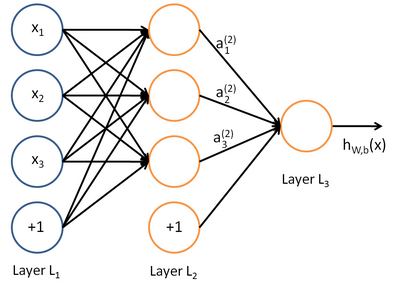
\includegraphics[width=120mm]{mnn.png}
    }
    \caption{Многослойная нейронная сеть}
    \label{figCurves}
  \end{figure}

Часто используемая функция активации - сигмоид:
  \begin{align}
	f(z_j)=\sigma(z_j)=(1+e^{-z_j})^{-1}
  \end{align}

Где:

  \begin{align}
	z_j=\sum{{w_{ij}}{x_i}}
  \end{align}

Полезное свойство сигмоида - её производная функции:
  \begin{align}
	\dd{\sigma}z=\sigma(z)(1-\sigma(z))
  \end{align}

Обучение такой нейронной сети производится обычно методом обратного распространения ошибки таким образом, чтобы минимизировать среднеквадратическую ошибку сети на обучающей выборке. Таким образом, обучающая выборка содержит пары векторов признаков (входные данные) и эталонных векторов (маркированные данные) {(x, y)}.

Метод обратного распространения ошибки:

Для выходного нейрона:
  \begin{align}
	\delta=z-y
  \end{align}

Для нейронов скрытых слоев:
  \begin{align}
	\delta_i=\sum_{j=0}^n \delta_j w_{ij}
  \end{align}

Коррекция весов:

Для выходного нейрона:
  \begin{align}
	w_{i0}'=w_{i0}+\eta\delta y_i
  \end{align}

Для нейронов скрытых слоев:
  \begin{align}
	w_{ij}'=w_{ij}+\eta\delta_j y_j(1-y_j)y_i
  \end{align}

В реальной практике, маркированных данных очень мало, для них требуется много сил и времени. Автоэнкодер представляет собой алгоритм обучения без учителя, который использует нейронную сеть и метод обратного распространения ошибки для того, чтобы добиться того, что входной вектор признаков вызывал выход сети, равный входному вектору, т.е. y = x.

Автоэнкодер явлается специальной архитектурой искусственных нейронных сетей, позволяющая применять обучение без учителя при использовании метода обратного распространения ошибки. Простейшая архитектура автоэнкодера — сеть прямого распространения, без обратных связей, наиболее схожая с перцептроном и содержащая входной слой, скрытый слой и выходной слой. В отличие от перцептрона, выходной слой автоэнкодера должен содержать столько же нейронов, сколько и входной слой.

  \begin{figure}[H]
    \noindent\centering{
        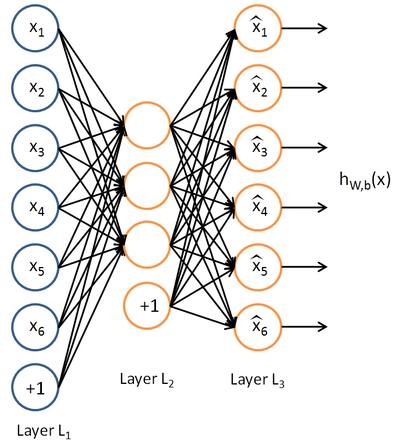
\includegraphics[width=120mm]{autoencoder.png}
    }
    \caption{Автоэнкодер}
    \label{figCurves}
  \end{figure}

Цель автоэнкодер - чтобы выход нейронной сети был наиболее близким к входному вектору. Для того, чтобы решение этой задачи было нетривиальным, на топологию сети накладываются особые условия:

1. Количество нейронов скрытого слоя должно быть меньше, чем размерность входных данных.

2. Активация нейронов скрытого слоя должна быть разреженной.

Первое ограничение позволяет получить сжатие данных при передаче входного сигнала на выход сети. Такая сжатие возможно, если в данных есть скрытые взаимосвязи, корреляция признаков или структура.

Второе ограничение – требование разреженной активации нейронов скрытого слоя, — позволяет получить нетривиальные результаты даже когда количество нейронов скрытого слоя превышает размерность входных данных. Будем считать нейрон активным, когда значение его функции передачи близко к 1 и наоборот, неактивным если значение его функции передачи близко к 0. Разреженная активация – это когда количество неактивных нейронов в скрытом слое значительно превышает количество активных.

Эти ограничения заставляют нейросеть искать обобщения и корреляцию в поступающих на вход данных, выполнять их сжатие. Таким образом, нейросеть автоматически обучается выделять из входных данных общие признаки, которые кодирутся в значениях весов сети.

Мы хотим, чтобы средняя активация каждого скрытого нейронна приняла значение, наиболее близкое к заданному разреженному параметру (порядка 0.05). Для этого, мы добавим в каждый нейрон скрытого слоя параметр разреженности $\rho$:

  \begin{align}
	\hat \rho_j=\frac{1}{m}\sum_{i=1}^m\biggl[a^{(2)}_j(x^{(i)})\biggl]
  \end{align}
  
  Мы хотим, чтобы средняя активация каждого скрытого нейронна приняла значение, наиболее близкое к $\rho$:
  \begin{align}
	\hat \rho_j=\rho
  \end{align}
  Штравная функция:
  \begin{align}
	S=\sum_{j=1}^{s_2}{KL({\rho}|{\hat{\rho_j}})}\\
	KL({\rho}|{\hat{\rho_j}})=\rho\log{\frac{\rho}{\hat{\rho_j}}}+(1-\rho)\log{\frac{1-\rho}{1-\hat{\rho_j}}}
  \end{align}
  Производная штравной функции:
  \begin{align}
	\dd{KL({\rho}|{\hat{\rho_j}})}{\rho_j}=-\frac{\rho}{\hat{\rho_j}} + \frac{1-\rho}{1-\hat{\rho_j}}
  \end{align}

\end{document}